\newcommand{\red}{\textcolor{red}{T1}}
\newcommand{\blue}{\textcolor{blue}{T4}}
\newcommand{\bluedrei}{\textcolor{blue}{T3}}
\newcommand{\tg}[1]{\textcolor{green}{#1}}
\newcommand{\cen}{\textcolor{orange}{\textbf{c}}}
\newcommand{\reda}{\textcolor{red}{a}}
\newcommand{\blueb}{\textcolor{blue}{b}}


\minpurp{Rotationen}
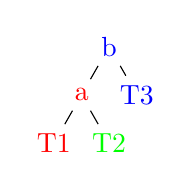
\begin{tikzpicture}[level distance=1.75em, sibling distance = 2em]
\node{ \blueb }
child{ node{\reda}
child{ node{\red}}
child{ node{\tg{T2}}}}
child{ node{\bluedrei}
}
;
\end{tikzpicture}
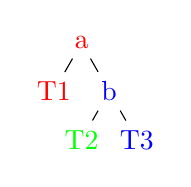
\begin{tikzpicture}[level distance=1.75em, sibling distance = 2em]
\node{\reda} 
child{ node{\red}}
child{node{\blueb}
child{ node{\tg{T2}}}
child{node{\bluedrei}}
};
\end{tikzpicture}

\quarterpage{ \centering
=> Rechtsrotation um a \\
<= Linksrotation um b
}



\minpurp{Doppelrotation}
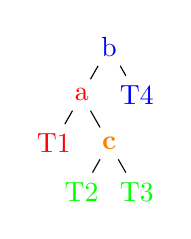
\begin{tikzpicture}[level distance=1.75em, sibling distance = 2em]
\node{\blueb} 
child{ node{\reda}
child{ node{\red}
}
child{ node{\cen}
child{ node{\tg{T2}}}
child{ node{\tg{T3}}}
}
}
child{ node{\blue}}
;
\end{tikzpicture} =>
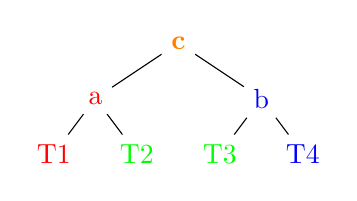
\begin{tikzpicture}[sibling distance=6em, level distance=2em ,level 2/.style={sibling distance=3em} ]
\node{\cen}
  child{ node{\reda}{
    child{ node{\red}}
    child{ node{\tg{T2}}}
  }}
  child{ node{\blueb}
    child{ node{\tg{T3}}}
    child{ node{\blue}}
  }
;

\end{tikzpicture} <=
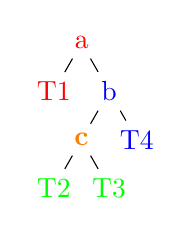
\begin{tikzpicture}[level distance=1.75em, sibling distance = 2em]
\node{\reda} 
child{ node{\red}}
child{ node{\blueb}
child{ node{\cen}
child{ node{\tg{T2}}}
child{ node{\tg{T3}}}}
child{ node{\blue}
}
}

;
\end{tikzpicture} 